% IEEE conference manuscript entry point.
% Adapted from IEEE's official conference-LaTeX template (June 2024).
% Keep the existing content/ hierarchy; write the paper in content/chapters/
% and place figures, tables, and bibliography records in their existing paths.
\documentclass[conference]{IEEEtran}

% Uncomment only when a funding acknowledgement is required in the first
% footnote. This command is part of the official IEEE template.
% \IEEEoverridecommandlockouts

\usepackage{cite}
\usepackage{amsmath,amssymb,amsfonts}
\usepackage{algorithmic}
\usepackage{graphicx}
\usepackage{textcomp}
\usepackage{xcolor}
\usepackage{booktabs}
\usepackage{hyperref}
\graphicspath{{content/images/}}

\begin{document}

\title{Paper Title}

% IEEE RCC 2027 uses double-blind review. Do not add author names,
% affiliations, emails, ORCIDs, acknowledgements, or identifying funding text
% to the review manuscript. Restore the IEEEauthorblockN/IEEEauthorblockA
% author block only for the camera-ready version.
\author{}

\maketitle

\begin{abstract}
Write a concise abstract for the target IEEE conference paper.
\end{abstract}

\begin{IEEEkeywords}
keyword one, keyword two, keyword three
\end{IEEEkeywords}

\section{Introduction}
\label{sec:introduction}

Aerial 3D scene understanding is central to autonomous uncrewed aerial vehicle (UAV) operation in cargo delivery, search and rescue, inspection, and human-UAV collaboration. In these settings, a perception system must infer not only visible image semantics, but also metric depth, free space, and the semantic occupancy of partially observed volumes. Semantic occupancy prediction combines partial visual observations with learned scene priors to infer the spatial structure and semantic composition of unobserved regions, supporting anticipatory action planning under uncertainty. These plans can be refined in real time as additional visual evidence becomes available. RGB cameras are attractive for UAVs because they are lightweight, inexpensive, and compatible with strict size, weight, and power constraints. However, monocular 3D perception remains difficult: image formation collapses scale, depth, and occlusion into a two-dimensional signal, and aerial views introduce altitude-dependent scale changes, oblique/top-down viewpoints, weak texture, and occlusion patterns that differ from ground-level driving scenes.

Most progress in semantic scene completion (SSC) and camera-based 3D perception has been driven by ground-level indoor and autonomous-driving benchmarks. SSCNet introduced semantic completion from depth input \cite{song2017sscnet}; MonoScene extended the task to monocular RGB \cite{cao2022monoscene}; and subsequent methods such as VoxFormer \cite{li2023voxformer}, TPVFormer \cite{huang2023tpvformer}, SurroundOcc \cite{wei2023surroundocc}, OpenOccupancy \cite{wang2023openoccupancy}, CGFormer \cite{yu2024cgformer}, and FoundationSSC \cite{chen2025foundationssc} improved view transformation, voxel attention, and semantic--geometric fusion. More recently, VoxDet reformulated voxel-wise SSC as dense object detection by decoupling semantic prediction from offset regression. Its training-free Voxel-to-Instance (VoxNT) transformation converts voxel-level semantic labels into six-direction object-boundary offset targets; the predicted offsets then guide instance-aware feature aggregation in the semantic branch \cite{li2025voxdet}. Together, these designs demonstrate the value of explicit 3D representations while showing that completion can benefit from both geometry-aware lifting and instance-aware voxel reasoning.

Existing aerial datasets provide valuable but complementary forms of supervision. UAVid focuses on 2D semantic segmentation of oblique urban imagery \cite{lyu2020uavid}; Mid-Air and SynDrone provide synthetic multimodal flights with depth and semantic labels \cite{fonder2019midair,rizzoli2023syndrone}; Dronescapes supports semantic segmentation, metric depth, and surface-normal estimation from real UAV video \cite{marcu2023dronescapes}; UrbanScene3D targets aerial path planning and multiview reconstruction \cite{lin2022urbanscene3d}; and UAVScenes combines image and LiDAR semantics with calibrated poses for several 2D and 3D perception tasks \cite{wang2025uavscenes}. These resources can benchmark segmentation, MDE, or reconstruction, but they do not directly provide the task-aligned dense semantic occupancy and free-space voxel ground truth required for SSC evaluation. OccuFly \cite{gross2026occufly} fills this gap by jointly providing real aerial RGB observations, metric depth maps, camera calibration and poses, altitude metadata, and semantic occupancy grids across multiple scenes and flight heights. We therefore use OccuFly to evaluate MDE, calibrated multiview geometry, and SSC under a common aerial protocol, asking whether modern foundation representations supply transferable geometric and semantic priors and whether neighboring views improve SSC beyond monocular depth and visual-context priors.

We study the transfer of frozen V-JEPA~2.1 and DINOv3 representations to aerial monocular depth estimation (MDE) and depth-aware semantic scene completion (SSC). Whereas V-JEPA learns by predicting latent representations rather than reconstructing pixels \cite{bardes2024vjepa,assran2025vjepa2}, V-JEPA~2.1 augments this objective with dense prediction over both masked and visible tokens and with deep self-supervision across encoder levels. The latter propagates local spatial information to the output representation, enabling the final encoder layer alone to support dense downstream prediction \cite[Secs.~2.3.1--2.3.2 and App.~9.1]{murlabadia2026vjepa21}. DINOv3 provides a complementary image representation optimized for dense visual transfer \cite{simeoni2025dinov3}. Using these frozen backbones, we examine how linearly accessible depth, multiscale decoding \cite{ranftl2021dpt,li2022vitdet}, camera-aware feature modulation \cite{perez2018film}, and temporal aggregation affect aerial MDE. We then assess how monocular and spatio-temporal visual priors, calibrated multiview geometry from a frozen MVSFormer++ depth estimator \cite{cao2024mvsformerpp}, and instance-aware voxel reasoning \cite{li2025voxdet} contribute to SSC. Only task-specific prediction and fusion modules are trained. Controlled comparisons isolate individual design factors, while repeated independent training runs quantify variability for the principal model; results for architectural controls evaluated without repetition are interpreted descriptively rather than causally.

Our evaluation has three parts. First, we compare linear probes, DPT-style multiscale decoders \cite{ranftl2021dpt}, Simple Feature Pyramid (SFP) adapters inspired by ViTDet \cite{li2022vitdet}, and Feature-wise Linear Modulation (FiLM) \cite{perez2018film} using altitude and camera intrinsics. This separates linear depth accessibility, dense reconstruction capacity, final-layer pyramid adaptation, and metric scale conditioning. Second, we compare RGB features with spatio-temporal V-JEPA~2.1 video features using a dense temporal-attention adapter that converts tubelet tokens into target-frame maps. Third, we evaluate SSC variants inspired by CGFormer and FoundationSSC, replacing or augmenting their geometry pathways with V-JEPA-derived depth probabilities and a pose-aware multiview stereo (MVS) cost-volume branch based on calibrated UAV views.

Our contributions are:
\begin{itemize}
    \item A systematic frozen-backbone evaluation of V-JEPA~2.1 RGB and video representations for aerial metric depth estimation on OccuFly.
    \item A controlled comparison of linear probes, DPT-style decoders, SFP-adapted final-layer decoders, and altitude/intrinsics-conditioned FiLM variants.
    \item An analysis of spatio-temporal feature transfer through dense temporal attention over V-JEPA~2.1 video tokens.
    \item A depth-to-SSC study that injects V-JEPA-derived depth maps and depth distributions into CGFormer- and FoundationSSC-inspired aerial SSC variants.
    \item A pose-aware FoundationSSC variant that replaces monocular depth lifting with calibrated multiview cost-volume depth estimation from neighboring UAV frames.
\end{itemize}

\section{Related Work}
\label{sec:related}

Frozen V-JEPA~2.1 and DINOv3 expose dense video- and image-pretrained features \cite{murlabadia2026vjepa21,simeoni2025dinov3}. DPT reconstructs dense predictions from several transformer levels, while FiLM conditions them by channel-wise affine modulation \cite{ranftl2021dpt,perez2018film}. Temporal aggregation alone does not establish correspondence: RAFT supplies optical-flow alignment \cite{teed2020raft,meister2018unflow}, whereas MVSFormer++ uses calibration, pose, and candidate depth in a cascaded attention-based MVS model \cite{cao2024mvsformerpp}.

CGFormer generates image-conditioned voxel queries, applies geometry-aware 3D deformable cross-attention, and combines voxel and tri-perspective representations \cite{yu2024cgformer}. FoundationSSC instead decouples foundation semantic features from stereo geometry, preserves probabilistic depth evidence, lifts complementary LSS and VoxFormer volumes, and merges them with Axis-Aware Fusion \cite{chen2025foundationssc,li2023voxformer}. VoxDet addresses a different stage: its spatially decoupled voxel encoder and task-decoupled predictor regress semantic-boundary offsets that guide classification \cite{li2025voxdet}. Symphonies and DISC provide further context/instance-oriented SSC references \cite{jiang2024symphonies,liu2025disc}. Our hybrid combines the FoundationSSC frontend with the VoxDet decoder; it does not claim equivalence to, or inherit efficiency claims from, either original system.

\section{Method}
\label{sec:method}

\begin{figure*}[t]
\centering
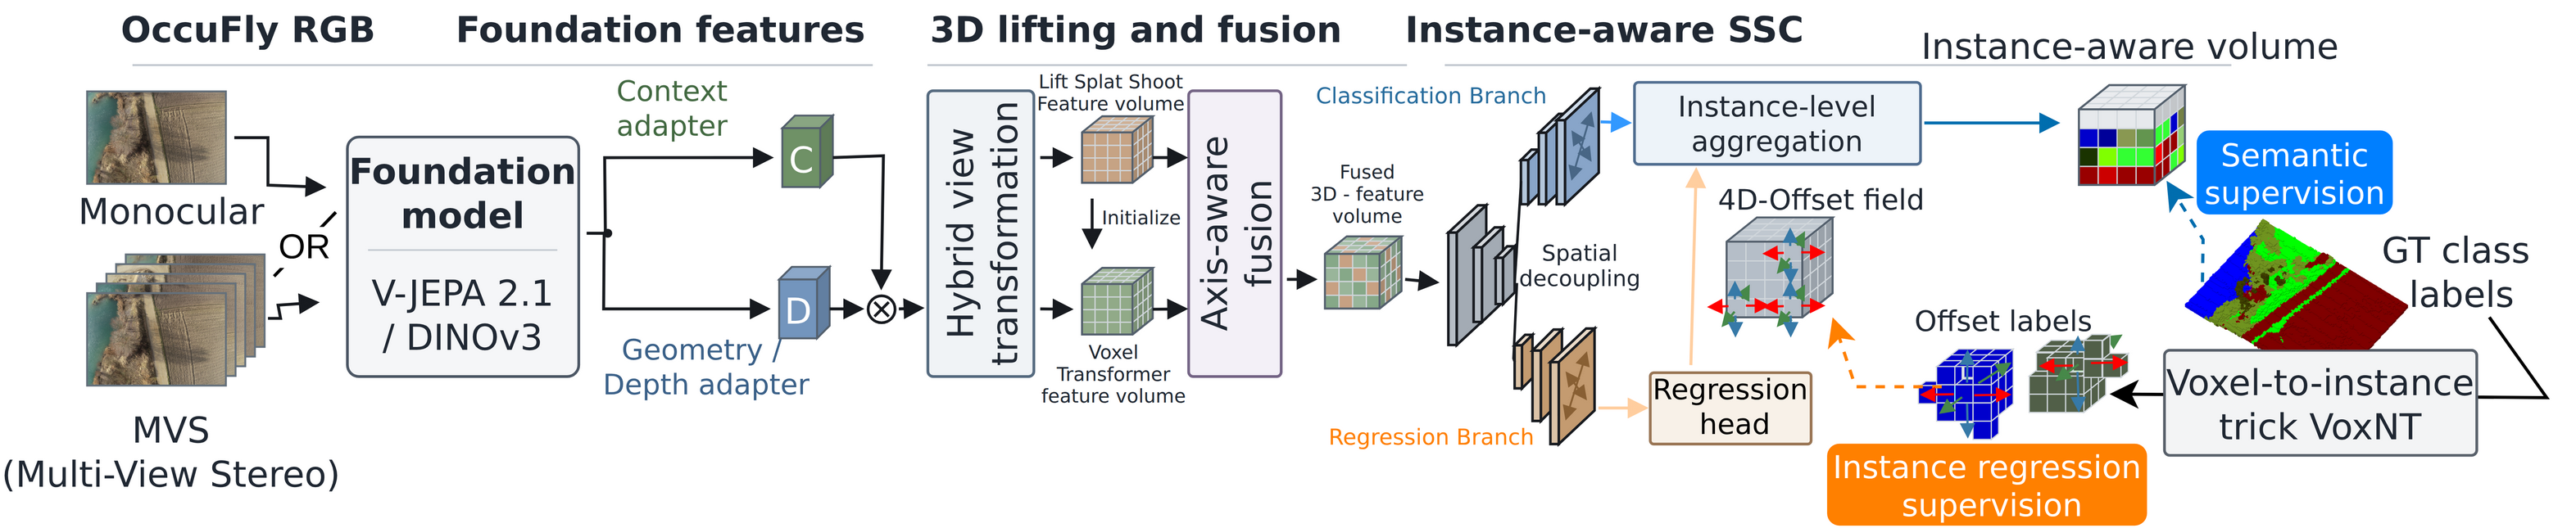
\includegraphics[width=\textwidth]{foundation_ssc_instance_pipeline.png}
\caption{Foundation-model pipeline for instance-aware semantic scene completion (SSC). Monocular or multi-view OccuFly RGB observations are encoded by V-JEPA~2.1 or DINOv3 foundation features. Context and geometry adapters feed hybrid-view 3D lifting and axis-aware fusion, followed by spatial decoupling into semantic instance aggregation and 4D offset regression branches. Semantic class labels and instance offsets provide the respective supervision signals.}
\label{fig:architecture}
\end{figure*}

We evaluate frozen foundation-model representations on two aerial 3D tasks: metric depth estimation and semantic scene completion (SSC). We select V-JEPA~2.1 and DINOv3 as complementary video- and image-pretrained representations and organize the framework as a sequence of depth-readout and SSC-decoder comparisons. For MDE, we compare final-layer linear probes with multilevel DPT-style dense decoders, and examine camera Intrinsics-altitude-aware FiLM conditioning, video-based dense temporal attention (DTA), pose-aware multiview matching, and native MVSFormer++ geometry. For SSC, we retain CGFormer as a monocular control and evaluate FoundationSSC-based variants that combine frozen V-JEPA~2.1 or DINOv3 context with FiLM-DPT monocular depth, calibrated MVSFormer++ geometry, or privileged GT depth, followed by either the retained FSSC voxel head or VoxDet decoding. Together with the MDE variants above, these configurations examine frozen-representation transfer, dense and metadata -conditioned depth decoding, temporal aggregation, geometry source, and voxel decoding. Concretely we seperate four questions: whether geometry is accessible from a frozen representation (RQ1), whether metadata helps beyond decoder capacity (RQ2), whether calibrated motion compensation improves temporal geometry (RQ3), and whether SSC is limited by depth, lifting, or semantic taxonomy (RQ4).

\subsection{Tasks and Information Pathways}
Each target observation has image $I_t$, intrinsics $K_t$, altitude $h_t$, and pose $T_t^{w\rightarrow c}$. Supervised training additionally uses depth $D_t$, its validity mask $M_t$, and semantic voxel labels $Y_t$. MDE predicts camera-axis depth $\hat D_t$ in meters. SSC predicts a categorical label $\hat Y_t(v)$ for each voxel $v$, with label zero representing empty space and labels 1--21 representing occupied semantic categories. Ground-truth (GT) depth and semantic labels supply supervision.

The pipeline separates context, geometry, and decoding. A frozen encoder supplies visual features. A context head maps those features to a semantic representation, while a geometry head or frozen MVS provider supplies depth information. A hybrid view transformer lifts context into a common voxel volume and fuses the resulting features. A voxel decoder then predicts occupancy and semantics. Figure~\ref{fig:architecture} shows these boundaries for depth transfer and the final multiview treatment. The division makes it possible to describe what changes across configurations without suggesting that every comparison isolates one factor.

For a target with neighboring views, define
\begin{equation}
\mathcal V_t=\{(I_i,K_i,T_i^{w\rightarrow c})\}_{i\in\{t\}\cup\mathcal S_t},
\end{equation}
where $\mathcal S_t$ contains source views. The monocular path uses only the target image and the metadata supplied to its head. The final multiview path uses one target and four calibrated sources. The temporal depth diagnostic uses a shorter target-centered neighborhood; it is a separate experiment and does not define the final SSC provider.

\subsection{Frozen Image Features}
The V-JEPA~2.1 ViT-Gigantic image encoder takes $384\times384$ inputs with patch size 16. It exposes $24\times24$ maps with 1664 channels. The four-level decoder reads zero-indexed blocks $\{11,23,37,47\}$; the last-layer probe reads block 47 alone. DINOv3 ViT-H+/16 uses the same target resolution and patch grid, with 1280-channel maps from blocks $\{7,15,23,31\}$.

Let $F_t^{(l)}=E^{(l)}(I_t)$ denote the selected frozen map. The foundation encoder is frozen: its features participate in the forward pass, but its parameters are not updated by gradients from the downstream task loss.

\begin{figure}[t]
\centering
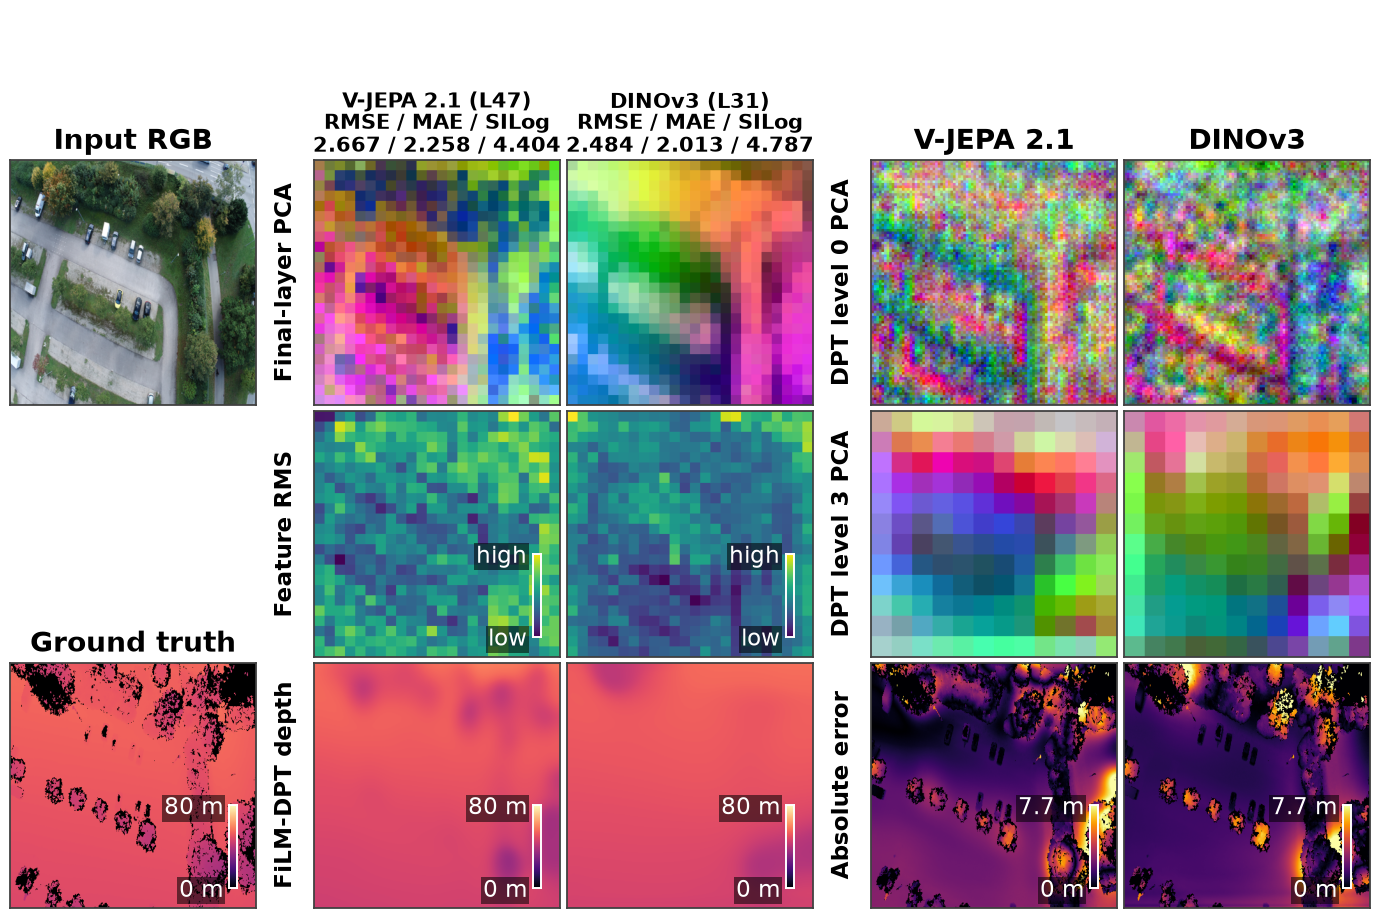
\includegraphics[width=\columnwidth]{vjepa_dinov3_feature_diagnostics.png}
\caption{Matched feature and depth diagnostics for V-JEPA~2.1 and DINOv3 on OccuFly scene~08 at 50~m (frame 000091). The final frozen maps are block~47 for V-JEPA and block~31 for DINOv3. DPT level~0 is the higher-resolution branch derived from the earliest selected backbone level and is architecturally positioned to retain finer spatial variation. Level~3 is the coarsest branch derived from the deepest selected level and has the largest effective context. These are architectural roles, not semantic interpretations of PCA colors. Each PCA is fitted independently and supports only within-panel inspection; colors are not comparable across models or levels. Feature RMS shows within-backbone activation magnitude using independently normalized low-to-high scales. }
\label{fig:backbone_feature_diagnostics}
\end{figure}

\subsection{Depth Heads and Metric Readout}
\subsubsection{Linear and DPT decoding}
The linear probe applies batch normalization and a $1\times1$ prediction layer to the final feature map. The head produces 256 depth-channel responses and a dense metric readout after spatial resizing. Its small capacity provides a baseline for geometry that can be extracted with limited adaptation.

The four-level DPT head projects selected maps into a common decoder representation and reassembles them at different spatial scales. Convolutional refinement progressively combines coarse and fine maps before depth prediction \cite{ranftl2021dpt}. Although all selected transformer maps have the same patch-grid size, their encoder depth differs; reassembly supplies the spatial pyramid needed by the dense decoder. The head therefore changes both the feature levels available and the reconstruction capacity relative to a final-layer linear probe.

\subsubsection{Depth-distribution readout}
At each pixel $u$, an image-depth head predicts $K=256$ responses
$z_{t,k}(u)$ associated with fixed metric-depth values $d_k$. A
head-specific nonnegative mapping followed by normalization produces
depth weights
\begin{equation}
p_{t,k}(u)=
\frac{a(z_{t,k}(u))}
     {\sum_j a(z_{t,j}(u))},
\qquad
\hat D_t(u)=\sum_k p_{t,k}(u)d_k .
\label{eq:depth}
\end{equation}
The reported image-depth map is therefore the expectation of the
discrete metric-depth representation. MVSFormer++ instead
returns an explicit categorical posterior over its native depth
hypotheses; for SSC, this posterior is projected onto the lifting grid
as described below.

\subsubsection{Camera-conditioned FiLM}
The metadata vector uses altitude and resized intrinsics:
\begin{equation}
m_t=\left[\frac{h_t-40}{10},\frac{f_x}{W},\frac{f_y}{H},
\frac{c_x}{W}-\frac12,\frac{c_y}{H}-\frac12\right].
\label{eq:metadata}
\end{equation}
A multilayer perceptron embeds $m_t$ into 128 dimensions. At each DPT level, channel-wise projections produce scale and shift vectors, giving
\begin{equation}
\widetilde R_l=R_l\odot(1+\gamma_l(m_t))+\beta_l(m_t).
\label{eq:film}
\end{equation}
The affine projections start near zero so the initial path remains close to the unconditioned decoder. Metadata thus modulates the interpretation of visual features while leaving the frozen encoder untouched. Camera conditioning enters only methods named FiLM-DPT.

\subsection{Temporal Aggregation and Pose-Aware Diagnostic}
\begin{figure*}[!t]
\centering
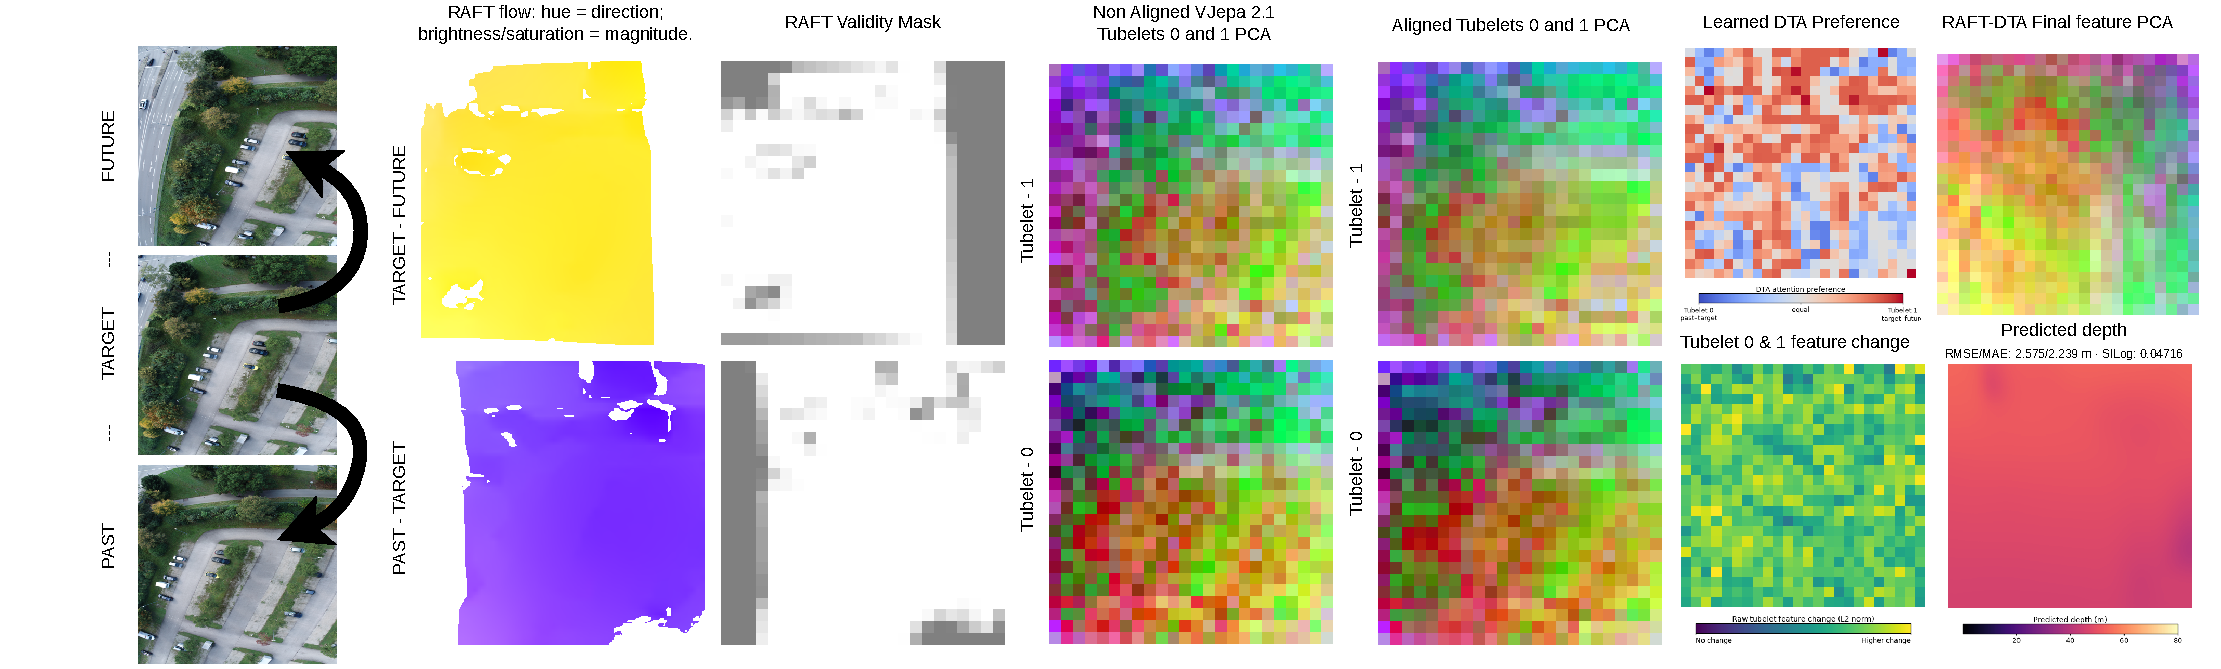
\includegraphics[width=\textwidth]{dtavideo/dta_raft_exact.pdf}
\caption{Flow-aligned DTA diagnostic for the four-frame V-JEPA~2.1 clip. The raw tubelet PCA maps precede alignment; feature change is their channel-wise $\ell_2$ difference, normalized at the 99th percentile. RAFT flow and validity backward-warp the past and future tubelets into target coordinates before DTA, whose blue/red preference favors tubelet 0/1. Raw, aligned, and DTA maps share one PCA basis; the predicted depth uses a 0--80~m scale.}
\label{fig:dta_raft_compact}
\end{figure*}

Video mode uses a four-frame clip with offsets $[-1,0,0,+1]$. The duplicated target yields an even length compatible with tubelet size two. Frame offsets are defined by sequence index, because measured capture timestamps are not available in the audited preprocessing records. The frozen video encoder returns two temporal tubelet positions at each spatial patch location.

A video linear adapter folds the tubelet dimension into channels. Dense Temporal Attention (DTA) instead learns a temporal readout separately at each spatial cell and each selected encoder level. With temporal tokens $G_{l,\tau}(u)$, the adapter has the form
\begin{equation}
\bar F_l(u)=\mu_l(u)+\alpha_l\bigl(A_l(G_l(u))-\mu_l(u)\bigr),
\label{eq:dta}
\end{equation}
where $\mu_l$ is temporal mean pooling, $A_l$ is learned-query attention, and the residual gate starts near mean pooling. The attention module uses a 512-dimensional adapter with eight heads. Its output has the same two-dimensional spatial form as an image feature map and can feed FiLM-DPT.

The implemented flow-aligned diagnostic addresses the same-cell assumption explicitly. Frozen RAFT \cite{teed2020raft} predicts target-to-frame flow $F_{t\rightarrow j}$ and reverse flow for every RGB frame. Out-of-view samples and forward--backward-inconsistent matches are invalidated \cite{meister2018unflow}. Because one V-JEPA token spans two frames, the two valid frame flows are averaged to obtain tubelet flow $\bar F_\tau$. For target coordinate $u$, source-tubelet features are then sampled as
\begin{equation}
\widetilde G_{l,\tau}(u)=G_{l,\tau}\!\left(u+\bar F_\tau(u)\right),
\label{eq:raft_warp}
\end{equation}
using bilinear backward sampling with \texttt{align\_corners=False}. The aligned DTA masks invalid tubelets in attention and replaces $\mu_l$ in Eq.~\eqref{eq:dta} by a validity-weighted mean. The aligned Linear Probe Video DTA control (MDE-2 in Table~\ref{tab:mde}) instead zeroes invalid samples before temporal concatenation, preserving a linear depth readout. RAFT, V-JEPA~2.1, and the warping operation are frozen or deterministic; only the downstream temporal adapter and depth head are trained.

Local temporal attention does not align features when the camera moves, because the same patch coordinate can correspond to different physical surfaces. The pose-aware component of Video DTA-FiLM-MVS (MDE-3 in Table~\ref{tab:mde}) therefore uses calibrated, depth-conditioned projective warping.

For homogeneous target pixel $\tilde u$ and depth hypothesis $d_k$, the target-camera point and its projection into source view $i$ are
\begin{equation}
x_{t,k}=d_kK_t^{-1}\tilde u,\qquad
q_{i,k}=\pi\!\left(K_i(R_{it}x_{t,k}+t_{it})\right),
\label{eq:projection}
\end{equation}
where
$T_{t\rightarrow i}
=T_i^{w\rightarrow c}(T_t^{w\rightarrow c})^{-1}
=[R_{it}\mid t_{it}]$
is the target-to-source camera transform and $\pi$ performs perspective division.

The source feature map is then warped into the target-view depth volume by bilinear sampling:
\begin{equation}
\widetilde F_{i,k}(u)
=
\operatorname{bilinear}\!\left(F_i,q_{i,k}\right).
\label{eq:mvs_warp}
\end{equation}
The warped source features are compared with the target features and combined across two source views to form a depth-indexed matching volume. A three-dimensional convolutional head regularizes this volume, and FiLM conditions the resulting depth responses. Unlike the preceding RAFT warp, this projective warp is determined by camera calibration, relative pose, and the tested depth hypothesis.

\subsection{Frozen Native Multiview Geometry}
The final multiview treatment (SSC-5 in Table~\ref{tab:ssc}) uses a frozen DINOv3-backed MVSFormer++ provider with one target and four calibrated source images. MVSFormer++ operates on $768\times1024$ images, while its foundation-feature branch uses $336\times448$ inputs. The retained geometry checkpoint is loaded strictly, and neither the DINOv3 backbone nor MVSFormer++ is updated during SSC training.

MVSFormer++ returns depth hypotheses $z_j(u)$ and their categorical probabilities $p_j(u)$. For our OccuFly SSC configuration, the LSS module discretizes camera-axis depth over $[0,64]$~m into $K=256$ bins of width 0.25~m, with centers $b_k$ from 0.125 to 63.875~m. This ray-depth discretization is distinct from the 0.5-m resolution of the OccuFly occupancy grid. We therefore linearly redistribute each MVS probability between its two neighboring lifting centers:
\begin{equation}
\widetilde P_k(u)=\sum_j p_j(u)w_k\!\left(z_j(u)\right),
\qquad
P_k(u)=\frac{\widetilde P_k(u)}
{\sum_l\widetilde P_l(u)} ,
\label{eq:posterior}
\end{equation}
where $w_k(z)$ is the linear interpolation weight for center $b_k$. Hypotheses outside the lifting range receive zero weight. If no probability remains within the range, the ray is marked invalid and does not contribute to lifting.

The context image is derived from the same target crop as the MVS input, with its intrinsics scaled to the corresponding resolution. This keeps the context features and projected depth posterior spatially aligned. Expected depth and photometric confidence are retained only as diagnostics; SSC lifting uses the complete projected distribution $P_k(u)$.

\subsection{Probability-Aware Lifting and Voxel Fusion}
The semantic context head consumes the target's frozen image features and produces a trainable DPT context map $C_t(u)$. For each image coordinate and lifting depth center, a camera ray maps context to a three-dimensional location. Schematically, the lift--splat contribution to voxel $v$ is
\begin{equation}
V(v)=\sum_{u,k}\mathbf1[\nu(x_{t,k}(u))=v]P_k(u)C_t(u),
\label{eq:lift}
\end{equation}
where $x_{t,k}(u)=b_kK_t^{-1}u$ and $\nu$ assigns a position to the configured voxel grid. Equation~\eqref{eq:lift} describes probability-weighted accumulation; the implemented hybrid view transformer additionally combines this dense pathway with proposal-guided voxel features and axis-aware fusion from the retained FoundationSSC modules.

The fused representation has 128 channels at $96\times64\times64$, corresponding to a reduced grid before full-resolution prediction. In the final multiview treatment, the retained view transformer and fusion pathway are frozen. Context and VoxDet decoding are trained while geometry and the lifting modules remain fixed. Context trains through the dense lift--splat and fusion path. Inputs to the frozen sparse voxel-attention branch are detached, preserving its forward features without backpropagating through that branch.

\subsection{VoxDet Decoding and VoxNT Targets}
VoxDet processes the fused volume with a shared three-dimensional encoder and task-specific branches. One branch predicts semantic features and logits, while another predicts six nonnegative directional offsets. Predicted offsets guide sampling and aggregation of semantic features along the voxel axes before final classification \cite{li2025voxdet}. The scored output remains a semantic occupancy grid. Directional predictions do not establish instance detection accuracy, and no instance average precision is claimed.

VoxNT generates supervision from semantic labels without learning additional parameters. For a voxel coordinate $i$ along an axis, the inclusive positive-direction run length is
\begin{equation}
r_+(i)=1+\mathbf1[Y(i)=Y(i+1)]r_+(i+1),
\label{eq:run}
\end{equation}
with terminal run length one. Applying the recurrence in both directions along three axes yields six targets. Each is normalized by its corresponding full-grid axis length. This is an axial same-label run, not Euclidean distance to the nearest object boundary or a connected-component box. A gap or class change ends the run, while touching same-label objects can remain indistinguishable.

Our implemented supervision enlarges predicted reduced-grid offsets to the full target grid and uses class-balanced Smooth-L1 loss with transition parameter 0.1. Eligible categories are tree, ground obstacle, person, bicycle, vehicle, building, cable, construction, crane, and truck. Losses are averaged within each present eligible class and then across those classes, reducing domination by large regions. All categories still receive semantic occupancy supervision. Target normalization uses the full-grid axis lengths before any resolution change.

Feature sampling uses the center-aligned coordinate
\begin{equation}
g(i;L)=2\frac{i+1/2}{L}-1
\label{eq:sample}
\end{equation}
for an axis of length $L$. This keeps voxel-center indexing consistent with the sampler's alignment convention. Tensor storage order is respected when coordinates are passed to the three-dimensional sampler. The treatment combines correct target scaling, consistent sampling, full-resolution supervision, and a long-tail objective; the available completed comparisons cannot assign its overall gain to one of these corrections alone.

Ground-truth VoxNT targets are used only during training. At inference, offsets are predicted from features, and no semantic target tensor is supplied. The phrase instance-aware describes the intended structural aggregation, with the semantic-label limitation above; it should not be read as verified separation of every physical instance.

\subsection{Occupancy and Long-Tail Semantic Objective}
Let $\ell_c(v)$ be the 22-class logit vector. Binary occupancy is trained from the stable occupied-versus-empty logit
\begin{equation}
\ell_{\rm occ}(v)=\log\sum_{c=1}^{21}\exp\ell_c(v)-\ell_0(v).
\end{equation}
A weighted binary cross-entropy (BCE) term supervises every valid voxel. Its positive weight is $\min(25,n_0/\sum_{c>0}n_c)$ from training counts. Conditional semantic focal cross-entropy is computed only at ground-truth occupied voxels, with focal exponent two. Semantic weights use square-root inverse training frequency, clipped to $[0.25,8]$ and then normalized to mean one over represented occupied classes. Empty voxels consequently supervise occupancy without overwhelming conditional category recognition.

A macro soft Dice term averages over semantic classes present in each batch. The main objective is
\begin{equation}
\mathcal L_{\rm main}=\mathcal L_{\rm occ}
+\mathcal L_{\rm focal}+0.5\mathcal L_{\rm Dice}.
\label{eq:mainloss}
\end{equation}
The auxiliary head uses corresponding weights $0.25$, $0.25$, and $0.10$, and full-resolution VoxNT has weight one. These weights are implementation settings rather than conclusions of a hyperparameter ablation.

The monocular VoxDet treatment additionally uses a metric-depth teacher term with weight 0.1 and a weak scheduled SSC-to-depth gradient. That gradient is zero in epoch zero, ramps over three epochs, and is capped at 0.1. Its purpose is to let the voxel decoder stabilize before limited adaptation of the pretrained depth head. The frozen multiview treatment has no depth loss and no such gradient schedule: its provider is run without gradients. All semantic, geometric, and offset masks exclude ignored labels. The distinction between these gradient paths is part of the method definition and limits direct architectural attribution from the final scores.

\definecolor{bestmiou}{RGB}{255,229,236}
\definecolor{bestiou}{RGB}{246,238,214}
\newcommand{\fsscrgbdirect}{FSSC RGB ctx DPT, depth FiLM-DPT}
\newcommand{\fsscrgbfilm}{FSSC RGB ctx FiLM-DPT, depth FiLM-DPT}
\newcommand{\fsscvidmvs}{FSSC video ctx DTA-DPT, depth DTA-MVS}
\newcommand{\fsscvidfilmmvs}{FSSC video ctx DTA-DPT, depth DTA-FiLM-MVS}

\section{Experimental Setup and Results}

\subsection{Dataset and Tasks}
We evaluate monocular depth estimation (MDE) and semantic scene completion (SSC) on OccuFly~\cite{gross2026occufly}. The standard split uses scenes 01--05 for training, scenes 06--07 for validation, and scenes 08--09 for testing across altitudes of 30, 40, and 50~m. The depth split contains 14,804 training frames, 1,965 validation frames, and 3,842 test frames. RGB inputs are resized to $384\times384$; metric depth is clipped to $[0.001,80]$~m and evaluated only over finite positive pixels that remain valid after mask-aware resizing. Video variants use consecutive frame-index neighborhoods because the released preprocess files provide frame indices and poses but no measured capture FPS.

For SSC, OccuFly labels are defined on a $192\times128\times128$ voxel grid in WHD order. The grid spans $x\in[-48,48]$~m, $y\in[-32,32]$~m, and $z\in[0,64]$~m, with 0.5~m voxels. Unless stated otherwise, experiments are run on an NVIDIA DGX node with 8 NVIDIA H100 80GB GPUs.

\paragraph{Controlled protocol and cost.}
Backbones are frozen; training updates only the named head. The matched V-JEPA/DINO comparisons use the same input resolution, official split, seed 0, per-GPU batch size 1 (global batch 8), 20-epoch budget, loss, and checkpoint criterion. Feature levels are matched by relative transformer depth. Exact decoder equality is impossible because V-JEPA~2.1 and DINOv3 expose 1664- and 1280-channel tokens: the corresponding linear heads contain 429,568 and 330,496 trainable parameters. DINOv3 ViT-H+/16 contains 840.6M frozen parameters. We report this deviation rather than projecting one backbone through an extra unmatched adapter. All current results are single-seed; margins are treated as descriptive until matched seeds are completed. Eight H100s accelerate the frozen-feature protocol but are not an onboard deployment claim.

\subsection{MDE Benchmarking Results}

Table~\ref{tab:mde_comparison} compares depth models on the standard OccuFly test split. We distinguish final test metrics from validation RMSE throughout. The historical plain-DPT row (11.471~m) was anomalous and its raw checkpoint is no longer auditable; we therefore replace it with the reproducible matched rerun (6.730~m). This correction reverses the earlier, implausible ordering: four-level DPT now improves over the last-layer linear probe. Under the matched FiLM-DPT protocol, DINOv3 reaches 4.358~m RMSE versus 4.770~m for V-JEPA~2.1, an 8.6\% reduction. DINOv3 also improves AbsRel, MAE, SILog, and $\delta_1$. The DINOv3 linear probe reaches 6.097~m RMSE, between the V-JEPA linear probe and the V-JEPA four-level DPT head, confirming that decoder capacity remains an important factor even with stronger frozen features. The pose-aware video checkpoint evaluated here is DTA-FiLM-MVS, not plain DTA-MVS: its multiview cost-volume output is FiLM-conditioned by altitude and intrinsics. It is evaluated on the 3,830 context-valid test frames, excluding the first and last frame of each scene--altitude sequence; the single-frame rows use all 3,842 test frames. We therefore report it as a diagnostic row and leave the unconditioned DTA-MVS ablation pending. Overall, these results show that the decoder and camera conditioning transfer across large frozen ViTs and that the strongest MDE result is not specific to V-JEPA~2.1.

\begin{table}[t]
\centering
\caption{OccuFly test MDE. In-house single-frame rows use frozen backbones at $384^2$ resolution and the official 3,842-frame scene split. DINOv3 rows match the V-JEPA training protocol for the corresponding head type. $\ddagger$ denotes the 3,830-frame context-valid subset used by the video MVS evaluator. Published DepthAnything2-OccuFly values follow OccuFly~\cite{gross2026occufly}. Dashes denote planned but unfinished runs. Best values are bolded per metric among completed rows.}
\label{tab:mde_comparison}
\resizebox{\linewidth}{!}{%
\begin{tabular}{lrrrrrrr}
\toprule
Method & $\delta_1 \uparrow$ & $\delta_2 \uparrow$ & $\delta_3 \uparrow$ & AbsRel $\downarrow$ & RMSE $\downarrow$ & MAE $\downarrow$ & SILog $\downarrow$ \\
\midrule
V-JEPA 2.1 linear probe & 0.651 & 0.959 & 0.997 & 0.188 & 7.795 & 6.447 & 0.225 \\
V-JEPA 2.1 four-level DPT & 0.747 & 0.970 & 0.997 & 0.162 & 6.730 & 5.411 & 0.200 \\
V-JEPA 2.1 FiLM-DPT & 0.816 & 0.970 & 0.998 & 0.131 & 4.770 & 3.457 & 0.166 \\
DINOv3 linear probe & 0.782 & 0.980 & 0.998 & 0.156 & 6.097 & 5.066 & 0.186 \\
DINOv3 FiLM-DPT & \textbf{0.848} & 0.968 & 0.998 & \textbf{0.121} & \textbf{4.358} & \textbf{3.209} & 0.161 \\
V-JEPA 2.1 DTA-MVS (pending) & -- & -- & -- & -- & -- & -- & -- \\
V-JEPA 2.1 DTA-FiLM-MVS$^\ddagger$ & 0.768 & 0.930 & 0.987 & 0.175 & 6.406 & 4.811 & 0.211 \\
\midrule
DepthAnything2-OccuFly~\cite{gross2026occufly} & \textbf{0.834} & \textbf{0.976} & \textbf{0.999} & 0.134 & 4.844 & 4.193 & \textbf{0.112} \\
\bottomrule
\end{tabular}
}
\end{table}

The previous altitude-interpolation table contained one method and reused scenes across altitude partitions, so it could not isolate conditioning from scene memorization. We retain that result only as an explicitly exploratory appendix diagnostic (Appendix Table~\ref{tab:occufly_depth_altitude_table12}); it is not used to support the FiLM claim. A valid causal comparison requires matched FiLM/no-FiLM heads and scene-disjoint training and testing.

Appendix Table~\ref{tab:mde_comparison_by_altitude} shows that the video FiLM-DPT branch is strongest at 30~m, while the RGB FiLM-DPT branch is stronger at 40~m and 50~m. The corresponding scene-wise breakdown is provided in Appendix Table~\ref{tab:mde_comparison_by_scene}: video helps on scene\_08, but RGB FiLM-DPT is stronger on scene\_09.

\subsection{SSC Benchmarking Results}

\paragraph{RQ4: Is low SSC accuracy primarily a geometry or taxonomy problem?}
OccuFly is extremely imbalanced: empty voxels dominate the grid, building is the largest occupied class, and several safety-relevant classes have only negligible support. Consequently, aggregate voxel accuracy can remain high while macro semantic IoU is low. Similar-looking structures further fragment supervision across fine labels (e.g., road/walkway/parking surfaces, or building/roof/construction), so errors can reflect semantic ambiguity in addition to lifting error. We therefore report SC IoU, GT-present SSC mIoU, fixed-denominator mIoU, frequency-weighted IoU, and per-class support rather than interpreting one headline number alone.

Table~\ref{tab:ssc_overall_comparison} restores the complete earlier comparison alongside the newly verified VoxDet ablations. Superscript $\dagger$ identifies ACCV26-era results produced by the earlier evaluator; the canonical VoxDet block is re-evaluated on one 3,842-frame manifest, with $\ddagger$ flagging checkpoints from interrupted training jobs. We keep the protocols visibly separated rather than treating their absolute values as directly comparable. Pose-MVS is evaluated separately because its earlier checkpoint was unavailable. Because absolute SSC mIoU remains low and several margins are small, we interpret these experiments as diagnostics of geometry, lifting, and taxonomy rather than as a state-of-the-art claim.

\begin{table}[t]
\centering
\caption{OccuFly test SSC comparison. $\dagger$ denotes results retained from the earlier ACCV26 evaluator. The canonical VoxDet rows use the same 3,842-frame test re-evaluation, one global confusion matrix, GT-present non-empty-class mIoU, and ignore label 255 excluded. $\ddagger$ marks a canonical test evaluation of a validation-selected checkpoint from a training job that stopped before its configured 20 epochs. Architecture names expose the changed context, geometry, and optimization components.}
\label{tab:ssc_overall_comparison}
\resizebox{\linewidth}{!}{%
\begin{tabular}{lrr}
\toprule
Method & SC IoU $\uparrow$ & SSC mIoU $\uparrow$ \\
\midrule
\multicolumn{3}{l}{\textit{Published OccuFly baselines}} \\
Symphonies~\cite{jiang2024symphonies} & 13.68 & 0.58 \\
DISC~\cite{liu2025disc} & 29.52 & 2.04 \\
\midrule
\multicolumn{3}{l}{\textit{Earlier ACCV26 context--geometry variants ($\dagger$)}} \\
CGFormer + DAV2 depth prior$^\dagger$ & 36.77 & 3.05 \\
CGFormer + FiLM-DPT depth prior$^\dagger$ & 36.51 & 3.31 \\
FSSC: RGB-DPT context + FiLM-DPT depth$^\dagger$ & 37.68 & 3.46 \\
FSSC: FiLM-DPT context + FiLM-DPT depth$^\dagger$ & 35.47 & 1.73 \\
FSSC: video DTA-DPT context + DTA-MVS depth$^\dagger$ & 24.55 & 0.17 \\
FSSC: video DTA-DPT context + DTA-FiLM-MVS depth$^\dagger$ & 32.55 & 2.36 \\
\midrule
\multicolumn{3}{l}{\textit{Canonical VoxDet component ablations}} \\
CGFormer + DAV2 depth prior & 9.93 & 1.37 \\
FSSC: RGB-DPT context + FiLM-DPT depth & 34.42 & 3.48 \\
VoxDet: ResNet context + FiLM-DPT depth & 38.85 & 2.85 \\
VoxDet: RGB-DPT context + FiLM-DPT depth & 38.87 & 3.47 \\
VoxDet V5-V2: RGB-DPT context + FiLM-DPT depth + full-res VoxNT + long-tail loss + scheduled depth gradients$^\ddagger$ & \textbf{45.77} & \textbf{4.62} \\
VoxDet V5-V2: RGB-DPT context + DAV2 geometry + full-res VoxNT + long-tail loss$^\ddagger$ & 44.82 & 4.35 \\
\bottomrule
\end{tabular}%
}
\end{table}

\paragraph{VoxDet/VoxNT finding.}
VoxNT predicts six-direction offsets toward local semantic structure and supplies a geometry-aware auxiliary signal before the final 3D decoding. Among the available canonical test artifacts, the strongest configuration is \emph{VoxDet V5-V2 + V-JEPA 2.1 RGB-DPT context + FiLM-DPT depth + full-resolution VoxNT + long-tail loss + scheduled depth gradients}, at 45.77 SC IoU and 4.62 SSC mIoU. The serialized checkpoint confirms the V-JEPA DPT context encoder and the RGB FiLM-DPT depth checkpoint; its validation-mIoU-selected epoch is 2. The matched DAV2-geometry configuration reaches 44.82/4.35 from validation-selected epoch~5. Its checkpoint explicitly records \texttt{geometry\_depth\_source=dav2\_teacher}, \texttt{depth\_lr=0}, and zero SSC-to-depth gradients, so this result is not attributed to FiLM-DPT geometry or scheduled depth gradients. Both test artifacts use the same 3,842-frame protocol, but both training jobs are incomplete relative to their configured 20 epochs: the FiLM-DPT history ends at epoch~8 and the DAV2 history at epoch~6. Their checkpoint-level test measurements are valid, while claims about the final 20-epoch training recipe require resuming or rerunning both jobs to completion. The larger completion gain than semantic gain remains consistent with VoxNT improving occupied structure while rare-class recognition is limited by supervision.

\paragraph{UAV11 remapping diagnostic.}
We additionally merge the 21 occupied labels into ten UAV-oriented semantic groups plus empty (UAV11): constructed structure, transport surface, natural ground, low vegetation, tree, ground/construction obstacle, vulnerable road user, vehicle, thin infrastructure, and water. With the full-res VoxNT, long-tail-loss, scheduled-depth-gradient architecture trained from scratch, the best validation SSC mIoU increases from 5.64 on the original fine taxonomy to 9.32 on UAV11; validation SC IoU is 29.42. This is not a like-for-like benchmark improvement because the label space changes. It instead demonstrates that part of the low fine-class mIoU comes from sparse support and visually overlapping subclasses. Rare merged groups can remain unresolved---the UAV11 vehicle group has only 53 validation voxels---so remapping reduces, but does not remove, the long-tail problem. Full mappings, supports, and per-class scores are provided in the supplement.

\paragraph{RQ3: Where do temporal features help?}
Across the current MDE and SSC geometry experiments, temporal aggregation has only a small and inconsistent effect. Video FiLM-DPT is strongest at 30 m and on scene 08, but RGB is stronger at 40/50 m and on scene 09. Uncompensated camera motion makes snapshot-token aggregation an ambiguous test of temporal representation quality; Pose-MVS therefore preserves view identity and explicitly warps source features with calibration. We do not conclude that temporal features are unhelpful in general. OccuFly provides short sampled neighborhoods rather than continuous video, so benefits may emerge for dense streams with stable temporal correspondence, motion history, or dynamic cues.

\begin{figure}[!htbp]
\centering
\includegraphics[width=0.98\linewidth]{content/images/ssc/scene_08_50_000097_mde_appended_ssc.png}
\caption{Qualitative OccuFly depth and SSC example for scene 08 at 50~m altitude, frame 000097.}
\label{fig:occufly_ssc_qualitative_scene_08_50_000097}
\end{figure}

\FloatBarrier

\section{Discussion and Limitations}
\label{sec:discussion}

\subsection{What the Completed Evidence Establishes}
The results answer the central research question at the level of completed configurations. Frozen representations support metric aerial depth when paired with trainable task heads. Dense decoding and camera-conditioned readout produce lower reported depth error than the corresponding small probes. The final combination of frozen DINOv3 context features, a frozen native multiview geometry provider, and VoxDet decoding yields a repeated occupied-space result, while its semantic macro score remains low. This separation is the principal empirical finding: recovering occupied structure does not by itself solve fine-grained aerial recognition.

Architecture attribution is more limited. The multiview treatment differs from the historical FoundationSSC control in decoding, objective, and optimization. The two monocular backbone records differ in pretrained depth quality and realized validation budget. No factorial experiment separately varies all these components with repeated matched controls. We consequently describe consistent directions and complete-treatment differences, avoiding claims that VoxNT, camera metadata, or MVS alone explains a specific percentage-point gain.

\subsection{Geometry Quality and Semantic Recognition}
A scalar depth metric measures visible surface error. SSC consumes geometry through projection, feature accumulation, volumetric fusion, and completion, then evaluates an extended voxel space. Errors near boundaries can place features in the wrong voxel even when average depth error is modest. Conversely, a posterior that spreads mass across plausible depths may support occupied coverage despite an imperfect expectation. These differences help explain why the depth and semantic rankings are not identical, but the present data do not measure their causal contributions.

The final method explicitly retains a categorical geometry posterior. This provides a richer interface than a single expected depth, especially when matching evidence admits multiple candidates. However, categorical probabilities should not be interpreted as calibrated epistemic or obstacle-risk uncertainty. The network and adapter assign normalized mass, while reliable risk estimation would require additional validation of calibration, coverage, and behavior under distribution shift. Out-of-range exclusion and invalid-ray masking preserve the adapter's geometric contract; they do not establish the accuracy of the retained posterior.

Semantic recognition has a separate supervision bottleneck. A class-balanced objective reduces domination by empty and large occupied regions, but it cannot create visual evidence or annotation support for every category. Zero true positives for person, bicycle, and cable persist despite explicit occupied-class weighting and eligible directional supervision. The failure could involve classification, voxel placement, object visibility, or their interaction. Further diagnosis requires per-target predictions and confusion analysis tied to the evaluated manifest rather than another aggregate score alone.

\subsection{Reading Long-Tail Scores Correctly}
The standard 21-class macro average uses a fixed denominator and assigns zero contribution to classes absent from the evaluated split. It is a stable reporting rule, not proof that recognition of every category was tested. Per-class N/A labels identify absent ground-truth support, while an observed zero remains a failure on a represented category. The same convention must carry through captions and comparisons.

The support figure describes the test distribution. Without split-wide train/validation histograms, we cannot establish whether a rare test category was also rare or absent in training. Appearance ambiguity, visibility, voxel size, geometry, and annotation can influence IoU alongside frequency. Per-target predictions and complete split counts are needed to distinguish these mechanisms.

\subsection{Repetition, Data Identity, and Generalization}
Aligning model and sampler seeds makes each independent run reproducible under its training contract. The three-seed sample standard deviation reports variability across those runs, with all other stated settings held fixed. It is not a confidence interval over environments and does not turn a one-run historical control into a repeated baseline. A paired comparison should repeat the control with the same declared seeds and compare differences on the same evaluation targets.

All experiments concern one aerial dataset with two test scenes and flight heights represented in training. The paper does not establish generalization to other camera systems, weather, terrain, altitudes, or geographic regions. Nearby frames also share content, so a large frame or voxel count should not be confused with a large number of independent environments. Additional datasets and scene-level analyses are needed before drawing broader conclusions about aerial foundation-model transfer.

\subsection{Implications for Robotic Use}
The completed system provides a useful occupied-space research result, but its deployment implications must follow the measured tasks. A landing or inspection planner may need correct recognition of people, vehicles, cables, and traversable surfaces. Persistent failures in represented categories prevent claiming such semantic reliability from the headline completion score. A dense completed volume can contribute hypotheses to a planner, while newly observed evidence should update those hypotheses; the current experiments do not evaluate a closed-loop planner or certify an unobserved region as free.

The five-view geometry input creates additional practical requirements: synchronized or consistently indexed observations, calibrated poses, source-view selection, and sufficient image overlap. Pose error, changing objects, weak texture, and occlusion can affect correspondence. Their sensitivity is not measured in this study. A benchmark configuration with retained calibration is not a demonstration that the same geometry will remain accurate with online UAV pose estimates.

Compute is another unresolved dimension. Freezing large encoders reduces training adaptation but leaves their inference cost. The multiview provider processes higher-resolution images, and SSC constructs a dense voxel representation. Offline training on eight H100s does not quantify latency, memory, energy, or throughput on embedded hardware. The published efficiency of an upstream decoder cannot be transferred to this hybrid without measuring the complete frontend, geometry, fusion, and decoding path.

\subsection{Focused Next Experiments}
The most informative follow-up is a repeated matched comparison of the geometry-family control and final decoder treatment, with one target manifest and a shared validation search window. This would separate variability of the complete treatment from variability of the baseline and permit paired descriptive differences. A subsequent component study could vary full-resolution offset supervision, the occupancy/semantic objective, and depth-gradient adaptation while preserving the remaining contract.

For depth, primary result recovery and shared-target evaluation should precede additional architectural claims. Equal-budget repeated image heads would clarify decoder and metadata effects, while a common context-valid target set would permit a temporal comparison. For semantics, per-target confusion analysis and complete split histograms would help distinguish sparse supervision from geometric or appearance failures. These are proposed experiments, not unfinished numeric results inserted into the current tables.

\section{Conclusion}
\label{sec:conclusion}
We studied frozen image/video foundation representations for aerial metric depth and semantic scene completion on OccuFly. The completed depth comparison supports trainable dense readout and explicit camera conditioning, with provenance limits stated for retained MDE records. Combining frozen DINOv3 features and native calibrated multiview geometry with VoxDet-style voxel decoding produces a stable occupied-space result across three independent runs. Standard 21-class semantic evaluation and class-wise support show that this geometric progress coexists with substantial unresolved category recognition. The evidence supports the complete transfer configuration and motivates matched repeated controls, stronger per-target provenance, and rare-class diagnosis before deployment claims are made.


% The starter bibliography file is intentionally empty. Keep this false until
% at least one cited entry has been added to content/references.bib; IEEEtran's
% BibTeX style does not accept an empty bibliography environment.
% Set \includereferencestrue before a manuscript build with citations.
\newif\ifincludereferences
\includereferencesfalse
\ifincludereferences
\bibliographystyle{IEEEtran}
\bibliography{content/references}
\fi

\end{document}
